% Created 2020-09-22 mar 09:50
% Intended LaTeX compiler: pdflatex
\documentclass[11pt]{article}
\usepackage[utf8]{inputenc}
\usepackage[T1]{fontenc}
\usepackage{graphicx}
\usepackage{grffile}
\usepackage{longtable}
\usepackage{wrapfig}
\usepackage{rotating}
\usepackage[normalem]{ulem}
\usepackage{amsmath}
\usepackage{textcomp}
\usepackage{amssymb}
\usepackage{capt-of}
\usepackage{hyperref}
\hypersetup{colorlinks=true,urlcolor=blue}
\usepackage{fancyhdr}
\fancyhead{} % clear all header fields
\pagestyle{fancy}
\fancyhead[R]{2-SMX:SOX}
\fancyhead[L]{Unidad 01: Introducción y Virtualización]}
\usepackage{wallpaper}
\ULCornerWallPaper{0.9}{../rsrc/logos/header_europa.png}
\CenterWallPaper{0.7}{../rsrc/logos/watermark_1.png}
\author{Angel Berlanas Vicente}
\date{\today}
\title{Unidad 01 - Introducción y Virtualización}
\hypersetup{
 pdfauthor={Angel Berlanas Vicente},
 pdftitle={Unidad 01 - Introducción y Virtualización},
 pdfkeywords={},
 pdfsubject={},
 pdfcreator={Emacs 26.3 (Org mode 9.1.9)}, 
 pdflang={English}}
\begin{document}

\maketitle
\tableofcontents


\section{Virtualización}
\label{sec:org87266a9}

La virtualización es la tecnlogía que nos permite trabajar con el \emph{Hardware}
como si fuera \emph{Software}. 

Vamos a ver esto con un pequeño ejemplo.

Cuando el programa que ejecutamos en un ordenador es relativamente simple, muchas
veces consiste en un único archivo ejecutable que cuando se lanza, realiza la función
que debe hacer y luego termina. Si deseamos actualizarlo, desinstalarlo, copiarlo, o 
lo que se necesite, es sencillo: \emph{basta con trabajar con el fichero}.

Sin embargo, incluso en los programas más simples, existen una serie de \emph{dependencias}, que 
tienen que ver con los diferentes Sistemas Operativos, las versiones de las librerias gráficas, 
las de acceso a disco, la gestión de los USB, etc. 

A medida que los programas van complicándose y haciéndose más y más complejos comienzan a tener
subsistemas y ficheros que son cargados dinámicamente para realizar determindas tareas (\texttt{.dll}).

Otros ficheros que son utilizados por parte del Software en ejecución son:

\begin{itemize}
\item Ficheros de datos.
\item Ficheros de configuración.
\item Imágenes: iconos, colores, etc.
\item \ldots{}
\end{itemize}

Al final la instalación de un Software medio incluye una serie de ficheros ejecutables, librerias, 
recursos y configuraciones que deben ser \emph{copiados} al Sistema Operativo destino para que se pueda
ejecutar.

El proceso no es sencillo y muchas veces no es posible realizar una \emph{vuelta al estado inicial}.

Si para el Software es complicado, para los Sistemas Operativos, que son piezas de Software que acaban
muy vinculadas al Hardware, la instalación, desinstalación y configuración es al menos igual de complicada,
\emph{si no lo és mucho más}.

Para los Administradores de Sistemas (\emph{aka.} vosotros :-), la realización de pruebas de instalación
es algo que haréis muy habitualmente.

En cursos posteriores veréis no solo que se debe de instalar y adapatar el Sistema Operativo
si no también todas las aplicaciones y servicios que forman parte de la solución.

Utilizando los Entornos de Virtualización, conseguimos emular el \emph{Hardware} para tratarlo
en estas pruebas (o incluso en la entrega final), como \emph{Software}. Nos permitirá, sobre un único 
soporte \emph{físico}, ejecutar diferentes entornos completos virtualizando:

\begin{itemize}
\item Discos Duros.
\item RAM.
\item Dispositivos de Entrada/Salida.
\item Configuraciones de conectividad (\emph{Networking}).
\end{itemize}

Iremos viendo más detalles de la Virtualización a lo largo del curso, ya que se trata 
de una de las herramientas más potentes para los Administradores de Sistemas.

\subsection{Guest y Host}
\label{sec:orgf7990bb}

A medida que vayamos leyendo documentación veremos muchas maneras de referirse a las máquinas virtualizadas y a los hypervisores. Una de las nomenclaturas que más puede aparecer son las palabras Guest y Host :

\textbf{Guest} (\emph{invitado}) es la máquina virtualizada, la que vive "dentro" de la máquina real.
\textbf{Host} (\emph{anfitrión}) es la máquina real, la que dispone de hardware real y virtualiza las otras.


\newpage
\section{Configuración de la red en los entornos virtuales}
\label{sec:orgd66cdd4}
En los sistemas de virtualización, sean cuales sean, uno de los recursos
más importantes que tendremos que administrar es la red. En los sistemas
de información, los servidores y los recursos compartidos entre las
máquinas se comunican a través de la red en la mayoría de los casos.
Para una correcta configuración de los Sistemas Operativos, es necesario
que adquiramos las destrezas y conocimientos que nos permitiran ajustar
la configuración de la red de nuestras máquinas. Ya sean Virtuales o
físicas.

Las posibilidades que veremos a continuación son aquellas que nos
permite VirtualBox, sin embargo estos mecanismos los podremos aplicar a
casi todos los sistemas de Virtualización
(\emph{Hyper-V,Proxmox,Docker,\ldots{}}). La manera de configurarlos será distinta
pero los conceptos son muy parecidos.

Cuando preparamos una máquina virtual, uno de los menús que nos muestra
Virtualbox es el de la red.

\begin{center}
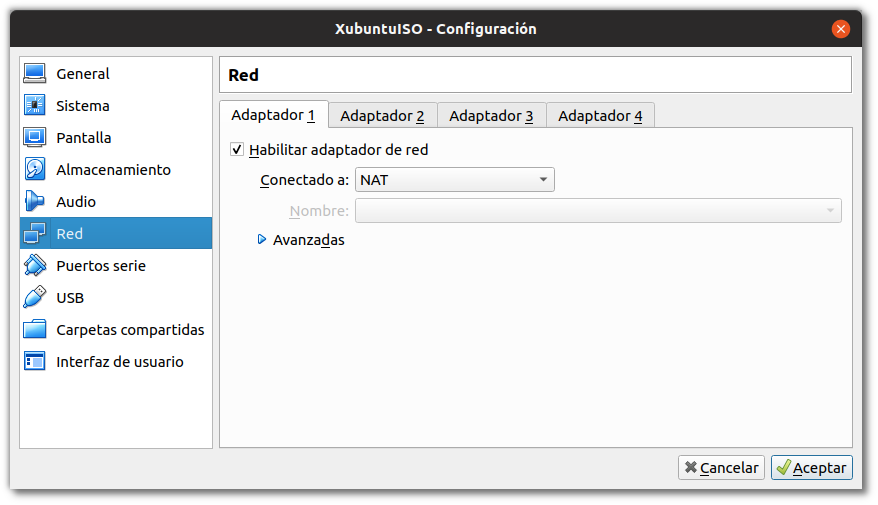
\includegraphics[width=.9\linewidth]{imgs/VBoxMenuRed_001_MenuInicial.png}
\end{center}

En este menú podemos configurar cual va a ser el modo en el que esa
máquina virtual podrá interactuar con la red a la que pertenece el
Hypervisor. Tal y como veremos a continuación existen varios nodos y
múltiples opciones, y deberemos seleccionar el que más se adecue a cada
uno de los casos en los que nos podremos encontrar.

\subsection{Hardware de Red Virtualizado}
\label{sec:orge992c8a}
Para cada una de las tarjetas de red que podemos conectar a nuestras
MVs, podemos seleccionar cual es \emph{modelo} de tarjeta que utilizaremos.

Los modelos disponibles son estos:

\begin{itemize}
\item AMD PCNet PCI II (Am79C970A);
\item AMD PCNet FAST III (Am79C973);
\item Intel PRO/1000 MT Desktop (82540EM) [/Por defecto/];
\item Intel PRO/1000 T Server (82543GC);
\item Intel PRO/1000 MT Server (82545EM);
\item Paravirtualized network adapter (virtio-net)
\end{itemize}

El modelo \emph{Paravirtualized network adapter} es especial ya que requiere
de un software adicional para la gestión de la red. Dejaremos el que
viene por defecto en la mayoria de los casos de este módulo.

\subsubsection{VirtualBox y los JumboFrames}
\label{sec:org78aae6f}
Si estamos utilizando \emph{Jumbo Frames} en nuestra red, es necesario que
utilizemos los modelos basados en Intel, ya que no tenemos soporte para
los mismos en el hardware Virtualizado de AMD. Sin embargo, esto lo
veremos más adelante en el tema de compartición de recursos en la red
(\textbf{NFS y SAMBA}) y estableceremos algunos parámetros que nos permitirán
trabajar con los recursos de la manera deseada.

\newpage
\subsection{No conectado}
\label{sec:org9a957c6}
En este modo VirtualBox le dirá al SO Virtualizado (\emph{Guest}) que tiene
una tarjeta de red pero esta no se encuentra \textbf{CONECTADA}, es decir es
como si no tuviera cable conectado. Esto será util para simular que la
red se ha desconectado, nuestro Switch se ha caido, o diferentes
ejercicios de simulación que podremos realizar.

\begin{center}
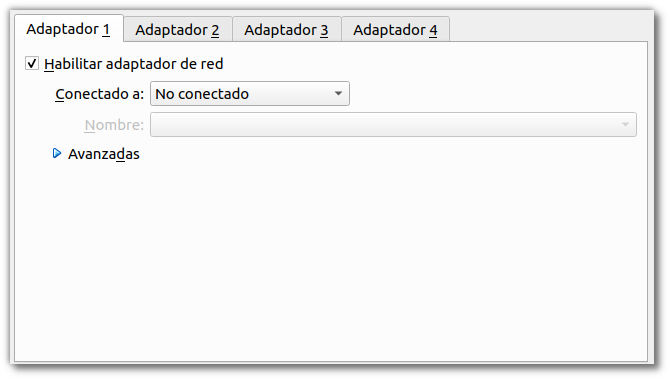
\includegraphics[width=.9\linewidth]{imgs/VBoxMenuRed_004_NoConectado.png}
\end{center}

\subsection{NAT}
\label{sec:orgc129426}
Network Address Translation (\textbf{NAT}) es el modo de conexión que viene por
defecto cuando creamos una máquina virtual. Si estamos configurando una
máquina para instalar cierto software, comprobar que todo funciona, o
para realizar pruebas que no tienen que ver con servicios de la red,
esta es la configuración más sencilla de utilizar.

En este modo, la IP asignada por defecto a la máquina es la :

\begin{verbatim}
10.0.2.15
\end{verbatim}

\begin{center}
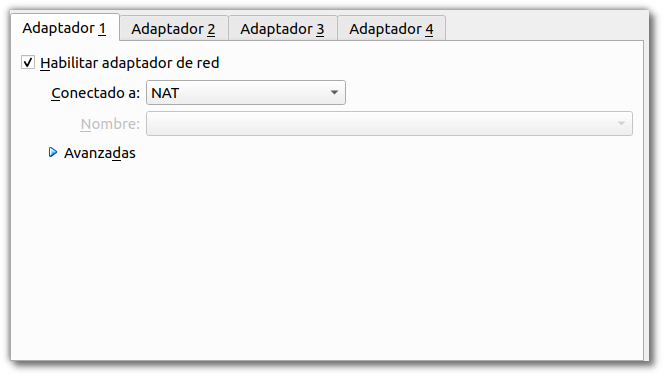
\includegraphics[width=.9\linewidth]{imgs/VBoxMenuRed_005_NAT.png}
\end{center}

\begin{center}
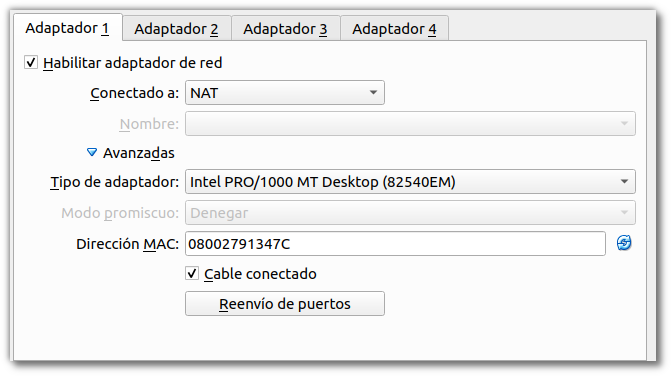
\includegraphics[width=.9\linewidth]{imgs/VBoxMenuRed_006_NAT_Ampliado.png}
\end{center}

Debemos tener en cuenta que en este modo tenemos algunas limitaciones
que pueden afectar a nuestras máquinas/pruebas. Podemos comprobarlo en
la página oficial del proyecto:

\begin{itemize}
\item\relax [[\url{https://www.virtualbox.org/manual/ch06.html\#nat-limitations}][VirtualBox
\begin{verbatim}
Limitaciones de NAT]]
\end{verbatim}
\end{itemize}

\newpage
\subsection{Red NAT}
\label{sec:orgc7ec01e}
Este servicio funciona de una manera similar a como funciona nuestro
Router en casa o en una pequeña empresa. Se agrupan los sistemas en una
red y se impide que los sistemas ajenos a ella (más allá del router)
puedan acceder directamente a ellos. Los sistemas que se encuentran
conectados mediante esta red pueden utilizar TCP y UDP sobre IPv4 e IPv6
para comunicarse.

Todas las máquinas que conectemos de esta manera serán capaces de
comunicarse entre ellas tal y como acabamos de comentar. La
configuración de esta red se realiza cuando se crea por primera vez.

\begin{itemize}
\item\relax [[\url{https://www.virtualbox.org/manual/ch06.html\#network\_nat\_service}][VirtualBox
\begin{verbatim}
Red NAT]]
\end{verbatim}
\end{itemize}

\begin{center}
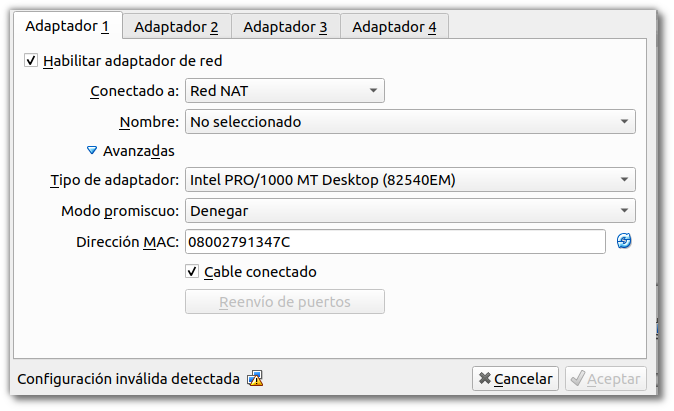
\includegraphics[width=.9\linewidth]{imgs/VBoxMenuRed_008_RedNAT.png}
\end{center}

\newpage
\subsection{Adaptador puente}
\label{sec:orgf15a769}
La configuración de adaptador puente nos permite interactuar con el
entorno de red del Hipervisor como si la Máquina Virtual se encontrara
en la misma Red. Genera una nueva interfaz de red por software,
accediendo a la red de manera física.

Si en nuestra red del Hipervisor tenemos un servidor de DHCP este le
asignará IPs a las máquinas que se encuentren conectadas de este modo,
permitiendo trabajar de manera conjunta a todas las máquinas, estén
virtualizadas o no, ya que para la red se encontrarán todas al mismo
nivel.

\begin{center}
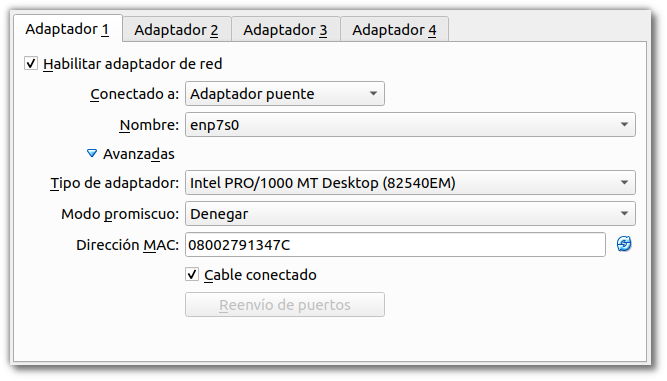
\includegraphics[width=.9\linewidth]{imgs/VBoxMenuRed_009_AdaptadorPuente.png}
\end{center}

\newpage
\subsection{Red interna}
\label{sec:orge9c68f1}
Cuando configuramos las máquinas virtuales en este modo, lo que
generamos es un \emph{switch} virtual al cual podemos ir conectando máquinas,
pero no podemos interactuar desde fuera del Hipervisor con esta red.
Servicios como DHCP no están en este modo por defecto, teniendo que
configurar todos los servicios de la red desde 0.

Podemos generar varias redes internas, que se crean automáticamente
cuando les cambiamos el nombre en el menú de configuración. Por defecto
el nobmre de la red interna es \textbf{intnet}.

Este será el modo de conexión cuando tengamos que configurar los
diferentes servicios que van asociados al dominio.

\begin{center}
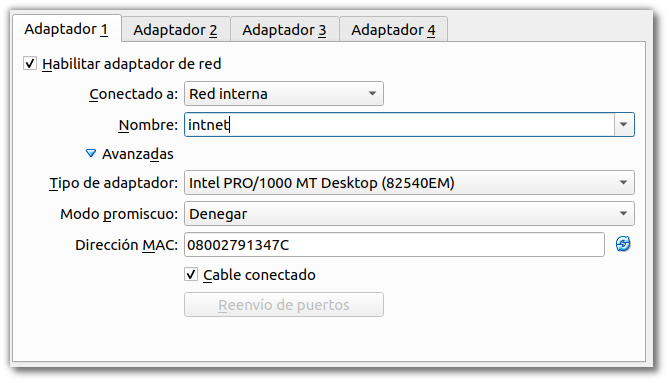
\includegraphics[width=.9\linewidth]{imgs/VBoxMenuRed_010_RedInterna.png}
\end{center}

\newpage
\subsection{Solo anfitrion}
\label{sec:org6d37909}
Se trata de una configuración de red que es un híbrido entre el modo de
\emph{Adaptador puente} y \emph{Red Interna}:

\begin{itemize}
\item Como \emph{Adaptador puente} las máquinas virtuales pueden hablar entre
ellas y con el hipervisor como si estuvieran conectadas mediante el
mismo cable físico.
\item Como \emph{Red Interna} , la interfaz de red interna no existe fuera del
hipervisor y no es posible contactar con las máquinas virtuales desde
fuera.
\end{itemize}

Cuando se utiliza este modo, VirtualBox crea una interfaz de red
mediante Software, que parece estar al lado de la tarjeta de red real
del hipervisor. Se trata de una dirección de red al estilo de
\textbf{loopback}.

Este modo es particularmente útil cuando estamos preconfigurando
sistemas que contienen un servicio o varios. Por ejemplo, una máquina
virtual podría contener un Servidor Web y otra un servidor de Base de
Datos, entre ambas deben poder comunciarse, el despliegue puede incluir
ordenes para el VirtualBox para que genere una red de \emph{Solo anfitrión}
que comunique ambas máquinas. Una segunda conexión de red mediante
\emph{Adaptador Puente} conectada a la máquina que tiene el Servidor Web, nos
permitirá acceder a esta desde cualquier máquina de la red del mundo
exterior al hipervisor, sin embargo no podremos acceder a la máquina con
el servidor de la Base de Datos.

\begin{center}
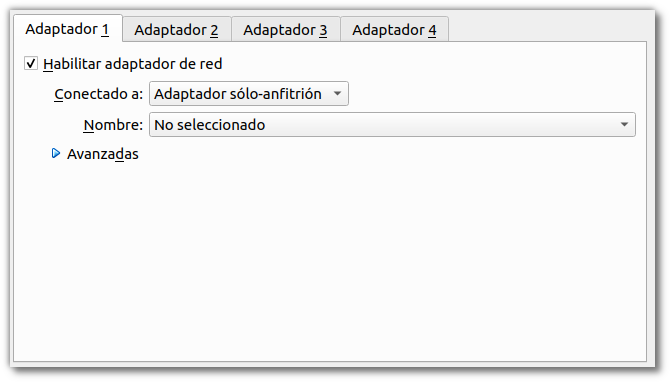
\includegraphics[width=.9\linewidth]{imgs/VBoxMenuRed_011_AdaptadorSoloAnfitrion.png}
\end{center}

\newpage
\subsection{Adaptador Genérico}
\label{sec:org923db1d}
Se trata de un modo similar al \emph{Adaptador Puente} pero permite al
usuario seleccionar el Driver que debe ser utilizado para emular esta
tarjeta.

\begin{center}
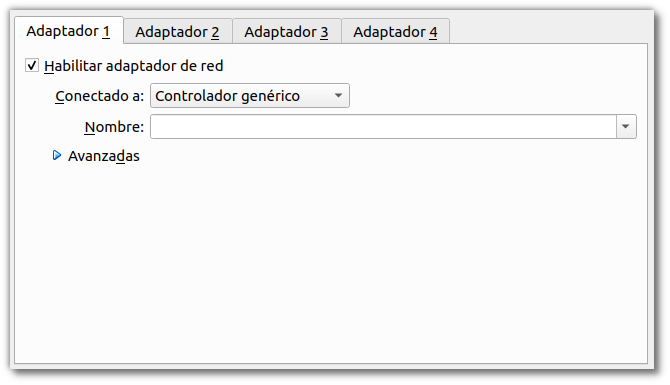
\includegraphics[width=.9\linewidth]{imgs/VBoxMenuRed_012_ControladorGenerico.png}
\end{center}

\newpage
\subsection{Enlaces sobre la red}
\label{sec:org247998e}
\begin{itemize}
\item \href{https://www.virtualbox.org/manual/ch06.html}{Manual de VirtualBox}
\end{itemize}


\newpage
\section{Recursos compartidos}
\label{sec:org795de0e}
Hemos visto como se gestiona la red y los recursos de red en los
sistemas de virtualización. Además de la red, existen otros como discos
duros USB, Carpetas Compartidas entre máquinas, audio de los sistemas
virtualizados, portapapeles, etc. que debemos saber configurar ya que
nos permitirán trabajar mejor y establecer mejores soluciones entre
sistemas.

\begin{center}
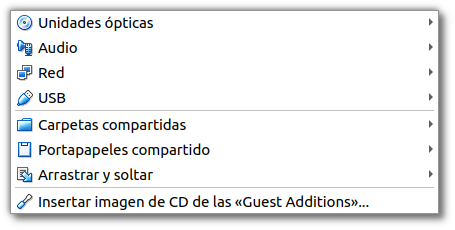
\includegraphics[width=.9\linewidth]{imgs/VBox_GuestAdd_LinuX_004.png}
\end{center}

\subsection{Permisos y vboxusers}
\label{sec:org8f4af84}
En GNU/LinuX el acceso a los diferentes dispositivos hardware por parte
de los usuarios (ya veremos más adelante todo esto en profundidad) está
gestionado mediante pertenencia a grupos de usuarios.

Cuando instalamos VirtualBox en GNU/Linux, este añade un grupo de
usuarios que es \textbf{vboxusers}, todos los usuarios que vayan a utilizar el
VirtualBox, si queremos tener acceso a todas las prestaciones y
operaciones posibles, debemos añadir ese grupo a los usuarios. Para
ello, bastará con que ejecutemos en el terminal:

\begin{verbatim}
sudo adduser NOMBRE_USUARIO vboxusers
\end{verbatim}

donde \texttt{NOMBRE\_USUARIO} es el \emph{login} del usuario que va a utilizar el
VirtualBox.

Una vez realizada esta operación es necesario reiniciar, ya que los
grupos y permisos son comprobados y establecidos durante el arranque de
la máquina.

\subsection{Audio}
\label{sec:org80ff256}
VirtualBox nos permite configurar el sistema de audio de la Máquina
Virtual para que suene a través del sistema de sonido del anfitrión
(Hipervisor).

\subsection{Puertos Serie}
\label{sec:org1c8166b}
Los puertos serie también pueden ser emulados dentro de las máquinas
virtuales, esto puede ser usado para hacer \emph{debug} o interactuar con
algunos sistemas cuyo mecanismo de comunicación no es el habitual.

\subsection{USB}
\label{sec:orgdeaced5}
Muchas veces cuando estemos trabajando con las máquinas virtuales
necesitaremos copiar algo \emph{dentro} o \emph{desde} una memória USB que
conectamos al hipervisor, así como configurar ciertos dispositivos
hardware dentro del sistema virtualizado.

En el menú de USB de la configuración de la MV podremos habilitar la
compatibilidad con los dispositivos USB. Por defecto el modo de
compatibilidad es 1.1, y este modo no nos dará ningún problema ya que
viene por defecto en todos los VirtualBox, sin embargo si deseamos
habilitar el USB 2.0 o el 3.0, se nos indica que debemos instalar el
\emph{Extension Pack} de VirtualBox para permitir el uso de este tipo de
dispositivos.

\begin{center}
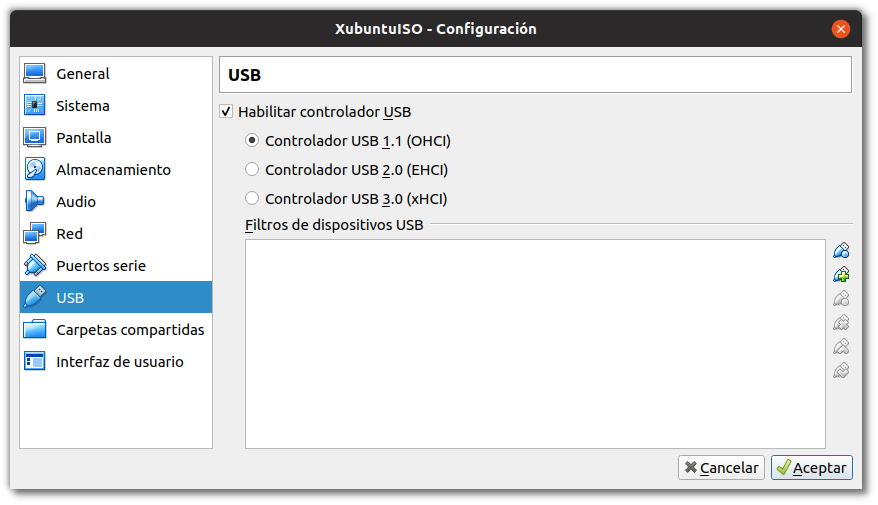
\includegraphics[width=.9\linewidth]{imgs/VBox_USB_1.png}
\end{center}

En caso de que no lo tengamos instalado en el hipervisor e intentemos
arrancar una máquina que si que tiene estas características habilitadas,
lo que ocurrirá es que no arrancará y nos mostrará un mensaje de error
acerca del USB.

\begin{center}
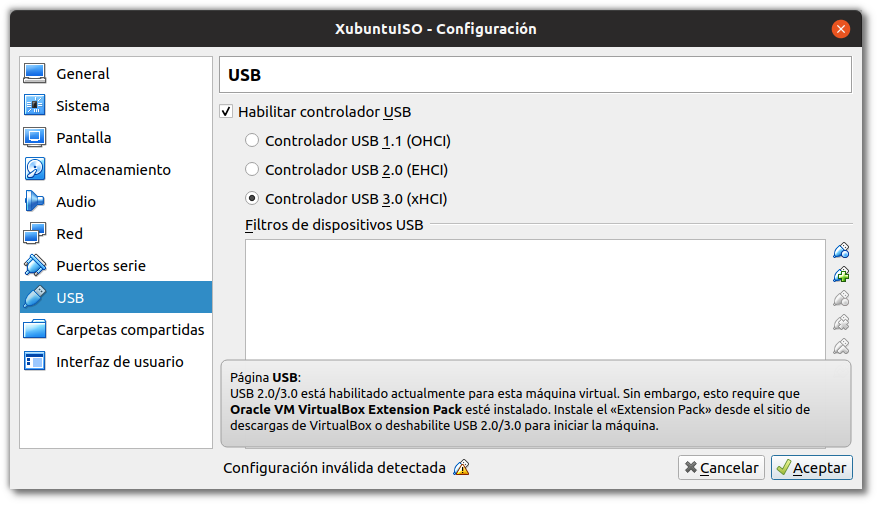
\includegraphics[width=.9\linewidth]{imgs/VBox_USB_2.png}
\end{center}

Los dispositivos USB que conectemos al VirtualBox, se dejarán de ver en
el hipervisor, ya que el módulo del VirtualBox se \emph{hará cargo} de los
dispositivos y no le permitirá al hipervisor administrarlos. Esto lo
tendremos que indicar en cada arranque de la máquina virtual, o
establecer un filtro. Esto lo veremos una práctica.

\subsection{Carpetas compartidas}
\label{sec:org64c5622}
Las carpetas compartidas es uno de los recursos más útiles que
encontraremos en el VirtualBox, ya que nos permitirá el paso de ficheros
cómodamente entre el hipervisor y el sistema virtualizado.

Veremos en una práctica como configurarlas, así como los permisos
necesarios para poder hacer uso de las carpetas en los sistemas
virtualizados.

Estas carpetas pueden estar configuradas para permitir tan solo
operaciones de lectura en los sistemas virtualizados, o configuradas en
modo lectura-escritura (bidireccional) de tal manera que nos permiten
pasar ficheros entre ambos sistemas, o más en el caso de que tengamos la
carpeta compartida entre varias máquinas virtuales en el mismo
hipervisor.


\newpage


\section{Tarea 06 : Compartir Recursos 1}
\label{sec:orgef2d342}

\begin{center}

\includegraphics[width=50px]{imgs/amongus.png}
\end{center}

Vamos a realizar una tarea en la que configuraremos una máquina Xubuntu
para que podamos compartir una serie de recursos entre el Hipervisor y
la máquina virtual.

Hemos visto en teoría que existen una serie de herramientas que nos
permiten mecanismos de comunicación entre la máquina virtual y el
hipervisor. No solo a través de la configuración de la red, sino también
herramientas útiles para el trabajo diario con estas máquinas virtuales:

\begin{itemize}
\item Establecer carpetas compartidas entre el \emph{Hipervisor} y la MV
\item La posibilidad de añadir texto \emph{enlaces}\ldots{} en el hipervisor y pegar
ese contenido en el sistema virtualizado (y \emph{viceversa}).
\item Permitir el uso de \emph{arrastrar y soltar} ficheros entre el Hipervisor y
la MV.
\end{itemize}

\begin{center}
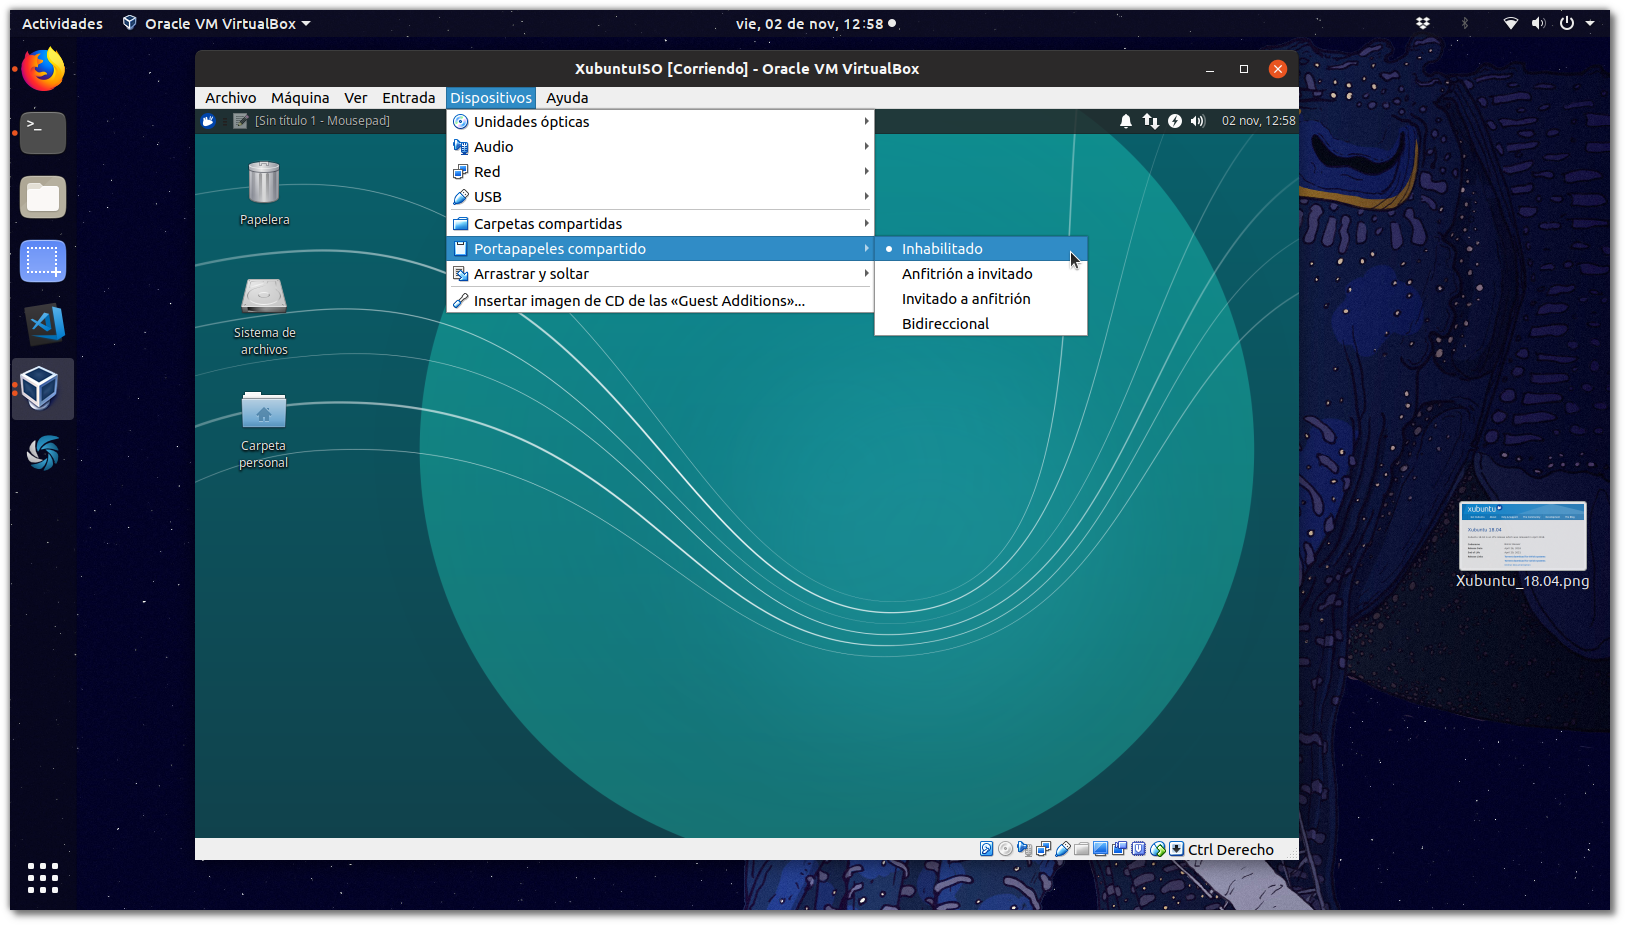
\includegraphics[width=.9\linewidth]{imgs/VBox_GuestAdd_LinuX_007.png}
\end{center}

\begin{center}
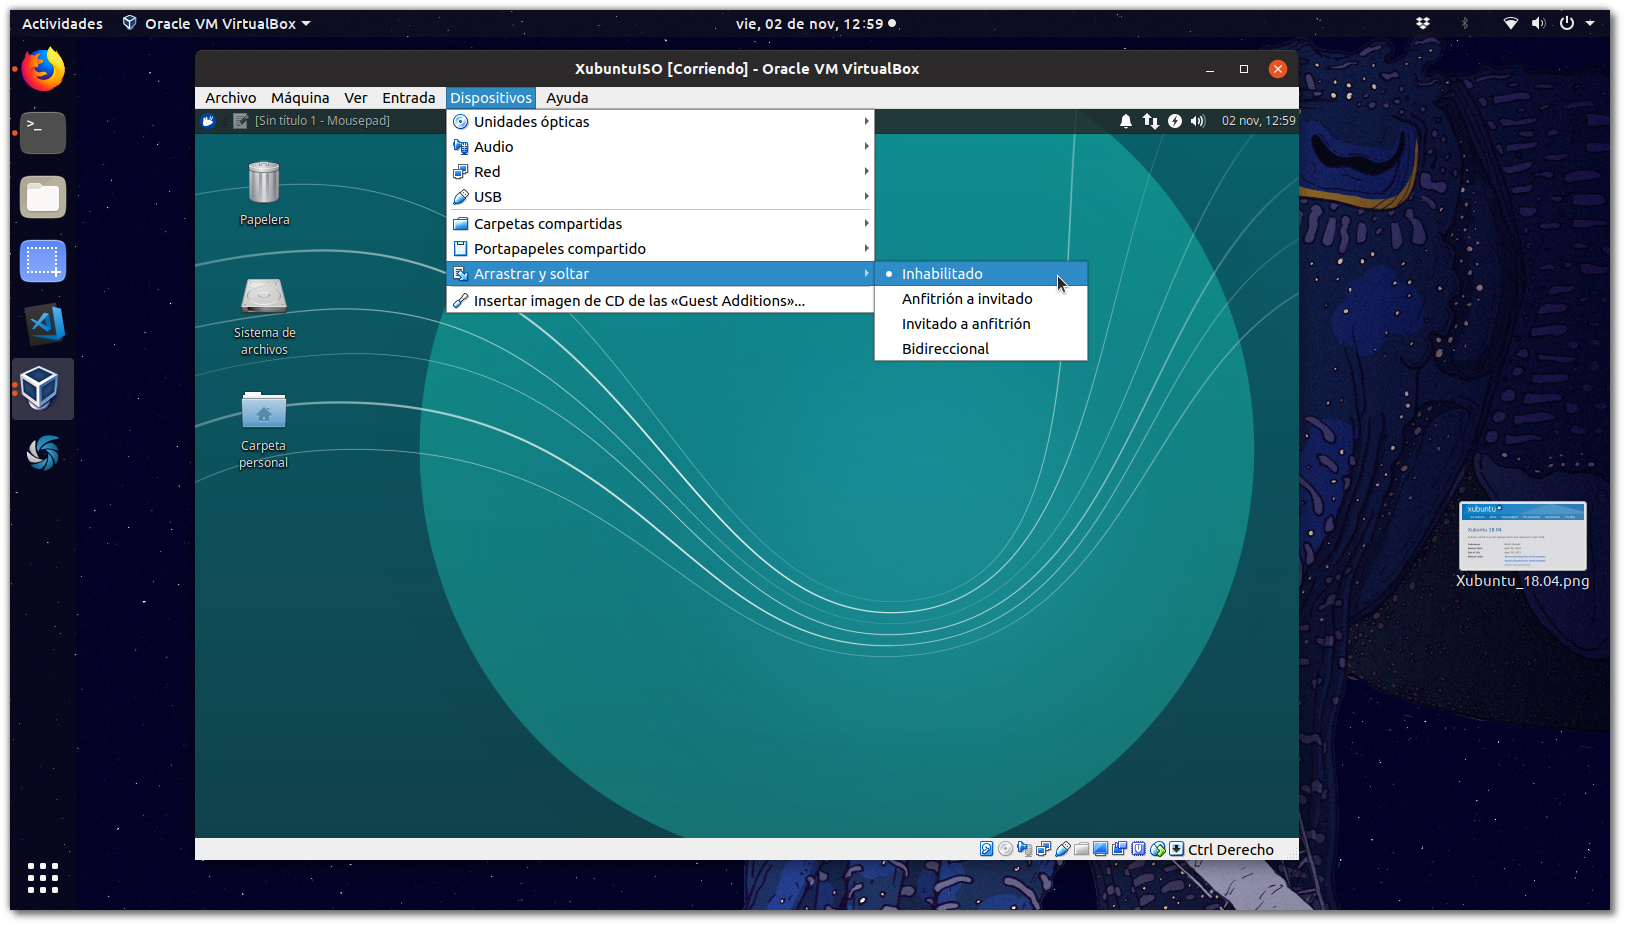
\includegraphics[width=.9\linewidth]{imgs/VBox_GuestAdd_LinuX_009.png}
\end{center}

Para poder utilizar todas las posibilidades que nos ofrece VirtualBox
para trabajar con las máquinas virtuales, utilizar memorias USBs en
nuestras máquinas, pasarnos ficheros, copiar y pegar del portapapeles
entre máquinas, etc. Necesitamos instalar en el sistema virtualizado una
serie de programas que le indican al sistema operativo virtualizado como
debe interactuar con esos recursos que le van a ser ofrecidos desde el
hipervisor.

Estos programas se denominan las \emph{Guest Additions} y a continuación
veremos una serie de pasos que se deben seguir para su instalación en
los sistemas GNU/LinuX. En el caso de los sistemas Microsoft Windows,
basta con que ejecutemos el \emph{autorun} que nos aparecerá cuando
insertemos el CD en nuestro sistema virtualizado.

\subsection{Instalación de las Guest Additions}
\label{sec:orgcc2165b}
En el menú \emph{Dispositivos} del VirtualBox y con la máquina virtual
encendida y con la sesión iniciada, activamos la opción:

\begin{verbatim}
Insertar imagen de CD de las <<Guest Additions>>...
\end{verbatim}

\begin{center}
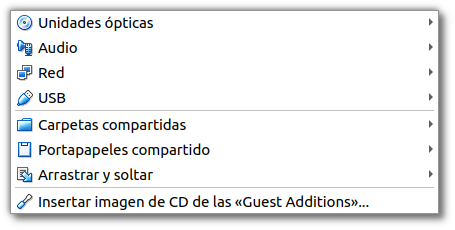
\includegraphics[width=.9\linewidth]{imgs/VBox_GuestAdd_LinuX_004.png}
\end{center}

Cuando lo hacemos en el sistema virtualizado nos aparece en el
Escritorio el icono del CD que acabamos de insertar (\emph{montar}), esto es
un comportamiento habitual en los Escritorios de GNU/LinuX.

Abrimos el CD y vemos el contenido de ese CD, podemos observar que hay
distintos ficheros, cada uno preparado para ser instalado en los
diferentes sistemas y arquitecturas habituales que se virtualizan:

\begin{itemize}
\item Windows (\textbf{32 bits})
\item Windows (\textbf{64 bits})
\item GNU/LinuX
\item Solaris
\end{itemize}

Lo que haremos será abrir una terminal aquí y ejecutaremos el instalador
para GNU/LinuX. Como funciona la terminal lo veremos más adelante en el
módulo, así como una explicación más detallada de las acciones que vamos
a realizar ahora, sin embargo son un buen punto de partida para
establecer un entorno de trabajo y pruebas más eficiente y cómodo.

\subsection{Instalando desde el terminal}
\label{sec:orgf67f2a0}
Para abrir un terminal, pulsaremos botón derecho en el explorador de
ficheros y seleccionaremos la opción: \textbf{Abrir un terminal aquí}.

\begin{center}
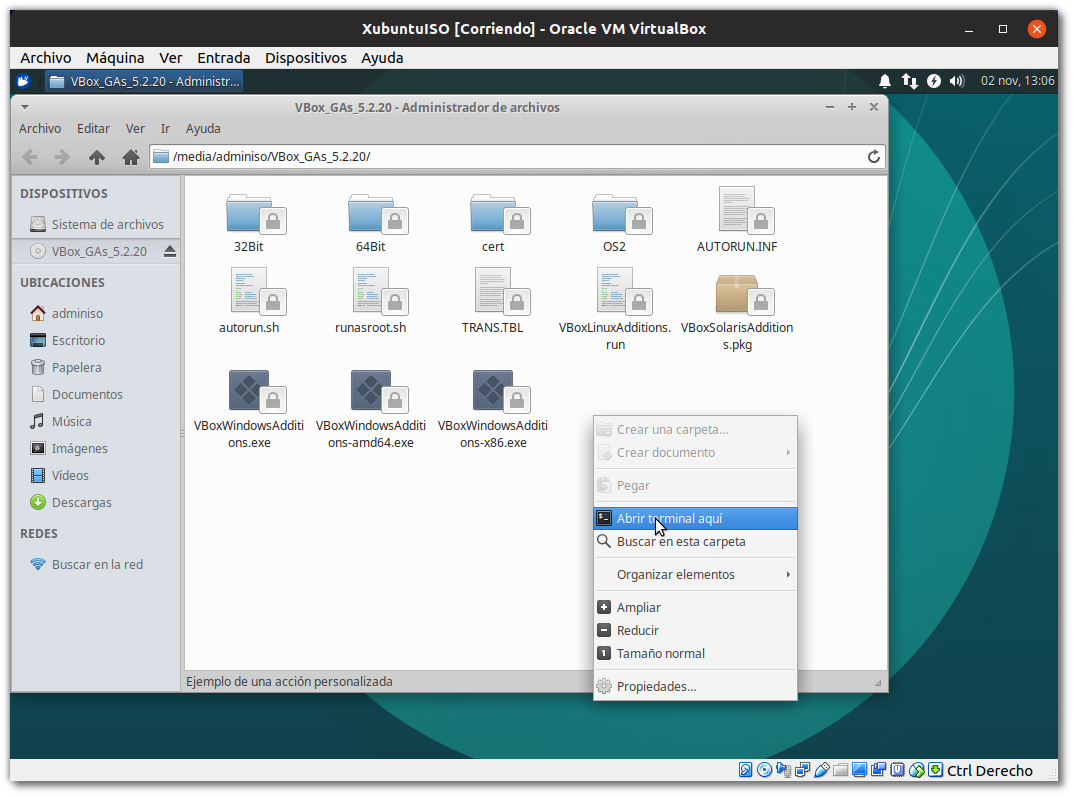
\includegraphics[width=.9\linewidth]{imgs/VBox_GuestAdd_LinuX_016.png}
\end{center}

Una vez abierto ejecutaremos el script de \emph{autorun.sh} que se encuentra
en la carpeta, para ello escribiremos en la terminal:

\begin{verbatim}
./autorun.sh
\end{verbatim}

\begin{center}
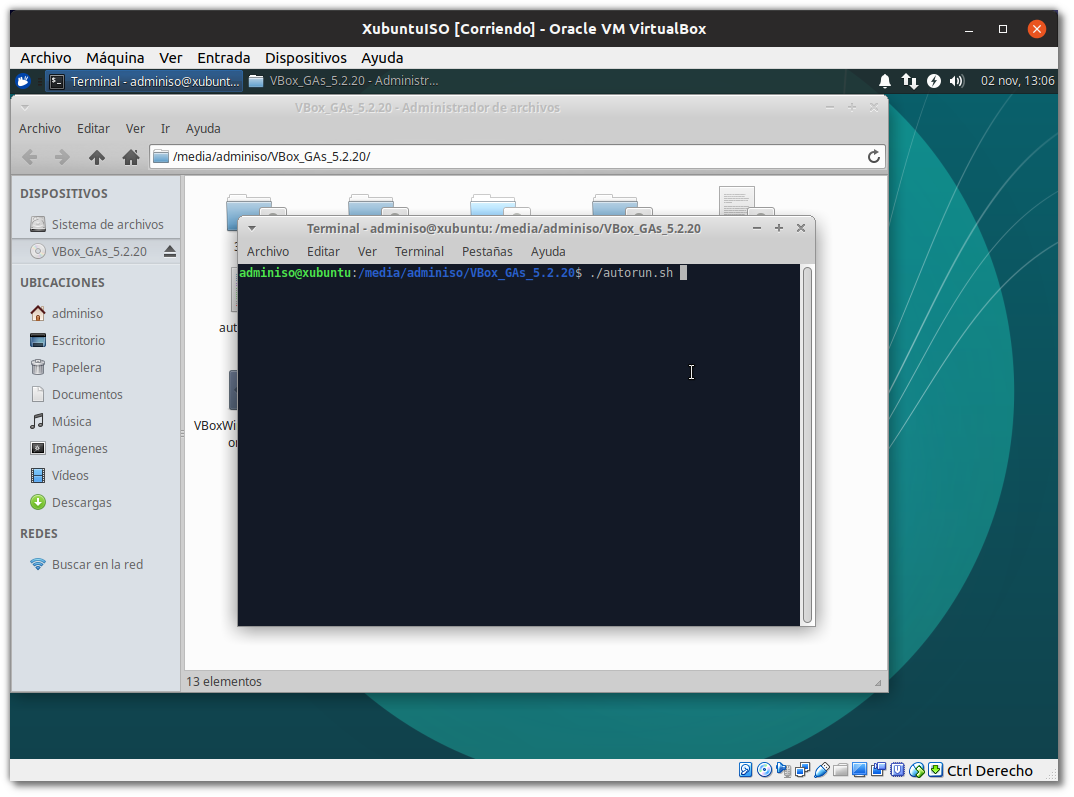
\includegraphics[width=.9\linewidth]{imgs/VBox_GuestAdd_LinuX_017.png}
\end{center}

Esta ejecución requiere de privilegios de administración, no sin motivo,
ya que en realidad estaremos configurando una serie de drivers que
tienen que ver directamente con nuestro Kernel (\emph{núcleo}) y con como van
a interactuar con ese hardware.

Introduciremos la contraseña de administrador.

\begin{center}
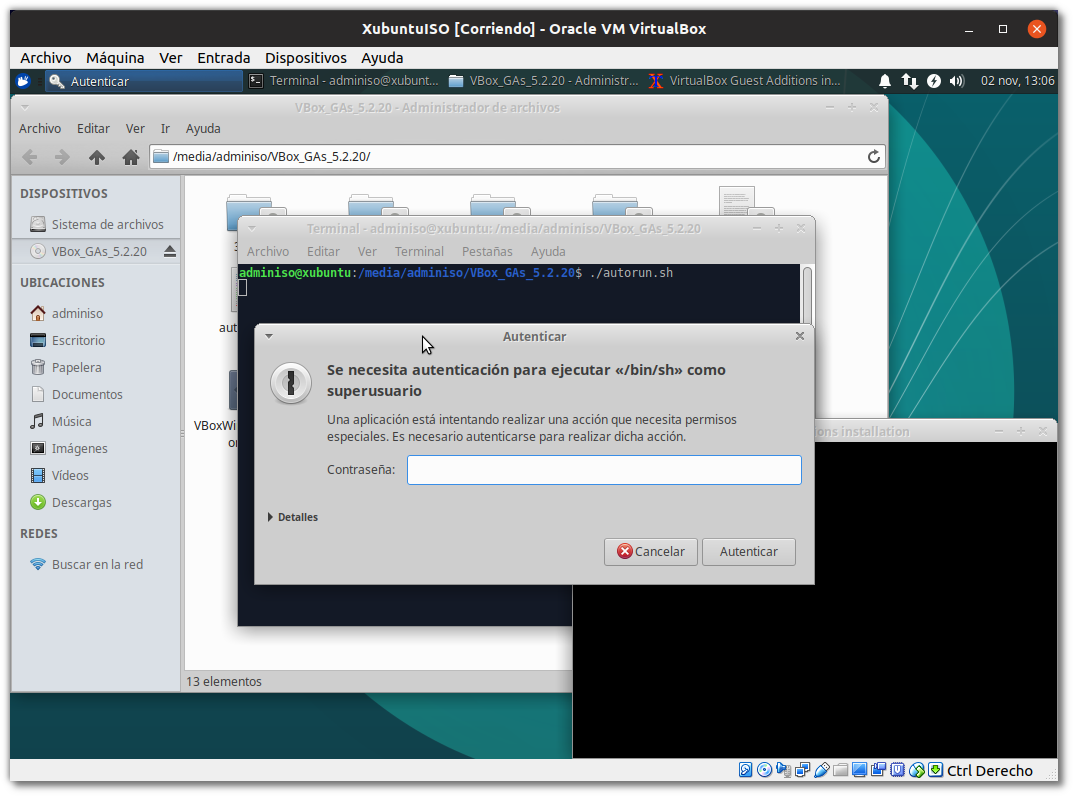
\includegraphics[width=.9\linewidth]{imgs/VBox_GuestAdd_LinuX_018.png}
\end{center}

Al ejecutarlo, nos aparece una pequeña terminal que nos muestra una
serie de mensajes acerca del progreso de la instalación, si leemos los
mensajes (y sí\ldots{}toca leer este tipo de cosas, más vale que nos vayamos
acostumbrando ya\ldots{}), nos daremos cuenta de que nos pide \emph{Por favor} que
instalemos : \emph{gcc, make y perl} para nuestra distribución.

\subsection{Instalando paquetes requeridos}
\label{sec:org33035ac}
Por ahora lo que haremos será ejecutar una orden en la terminal que nos
descarga los paquetes desde los repositorios y nos los instala. Esto lo
veremos con mucho más detalle en temas futuros, pero lo vamos a
necesitar ahora.

\begin{verbatim}
sudo apt install gcc make perl
\end{verbatim}

\begin{center}
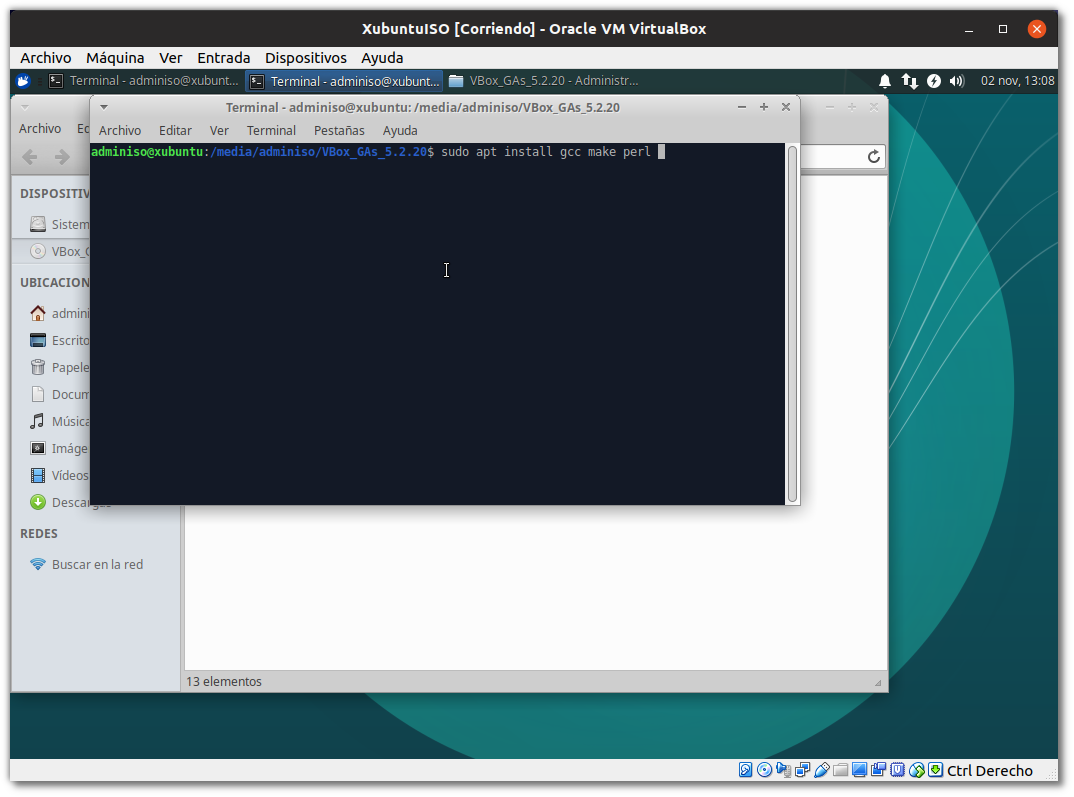
\includegraphics[width=.9\linewidth]{imgs/VBox_GuestAdd_LinuX_020.png}
\end{center}

A continuación nos muestra que se van a instalar una serie de paquetes y
nos pide confirmación, tal y como vemos en la imágen.

\begin{center}
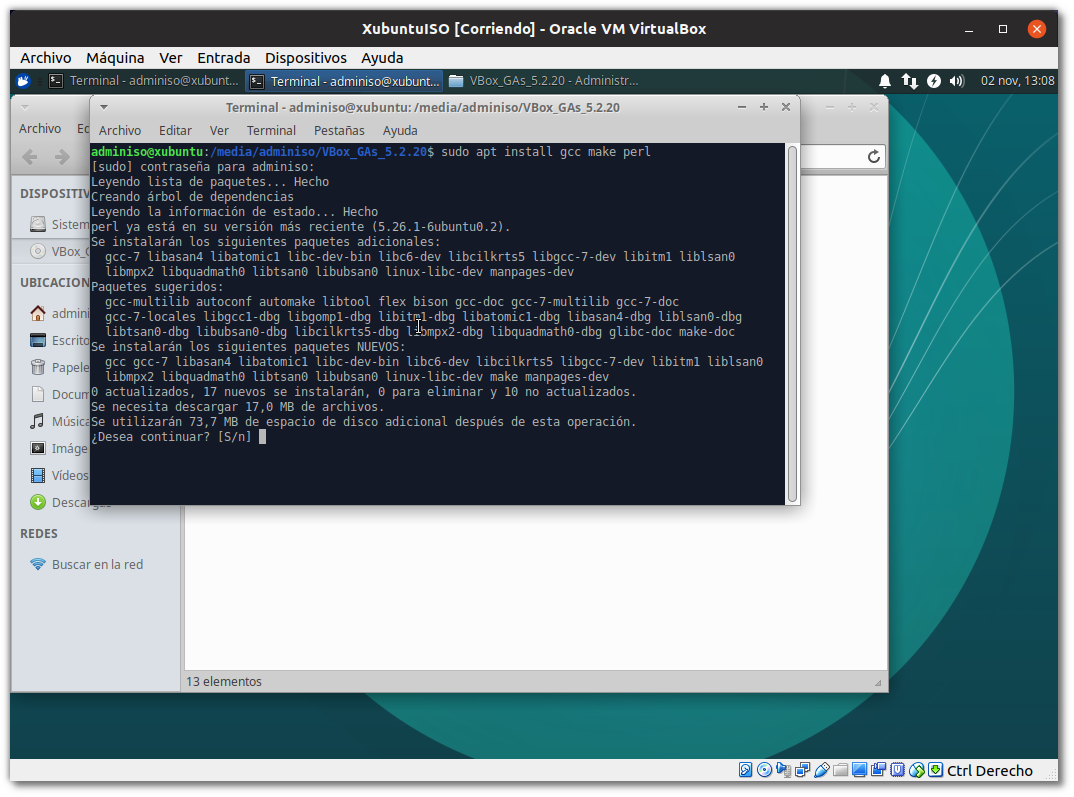
\includegraphics[width=.9\linewidth]{imgs/VBox_GuestAdd_LinuX_021.png}
\end{center}

\subsection{Continuamos la instalación}
\label{sec:org43a92b0}
Ahora si volvemos a ejecutar el script de \emph{autorun.sh} no nos dará
ningún mensaje de error.

\begin{center}
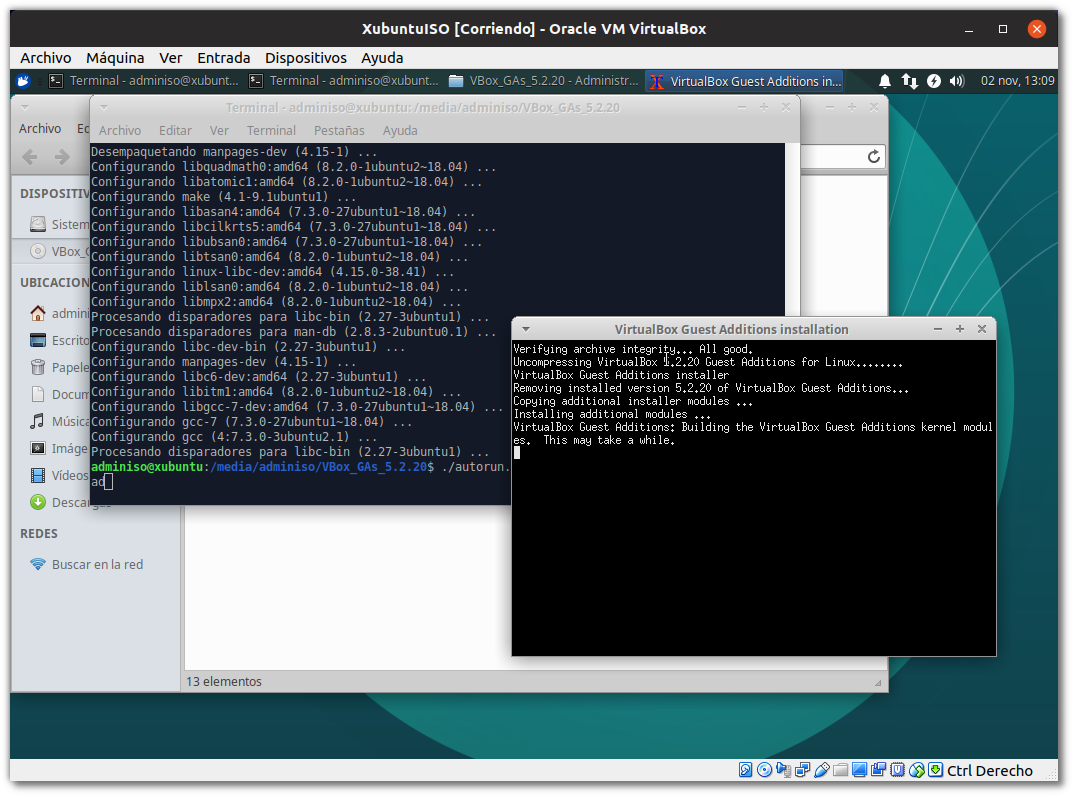
\includegraphics[width=.9\linewidth]{imgs/VBox_GuestAdd_LinuX_023.png}
\end{center}

Una vez realizado este paso, es conveniente reiniciar el sistema
virtualizado.

\begin{center}
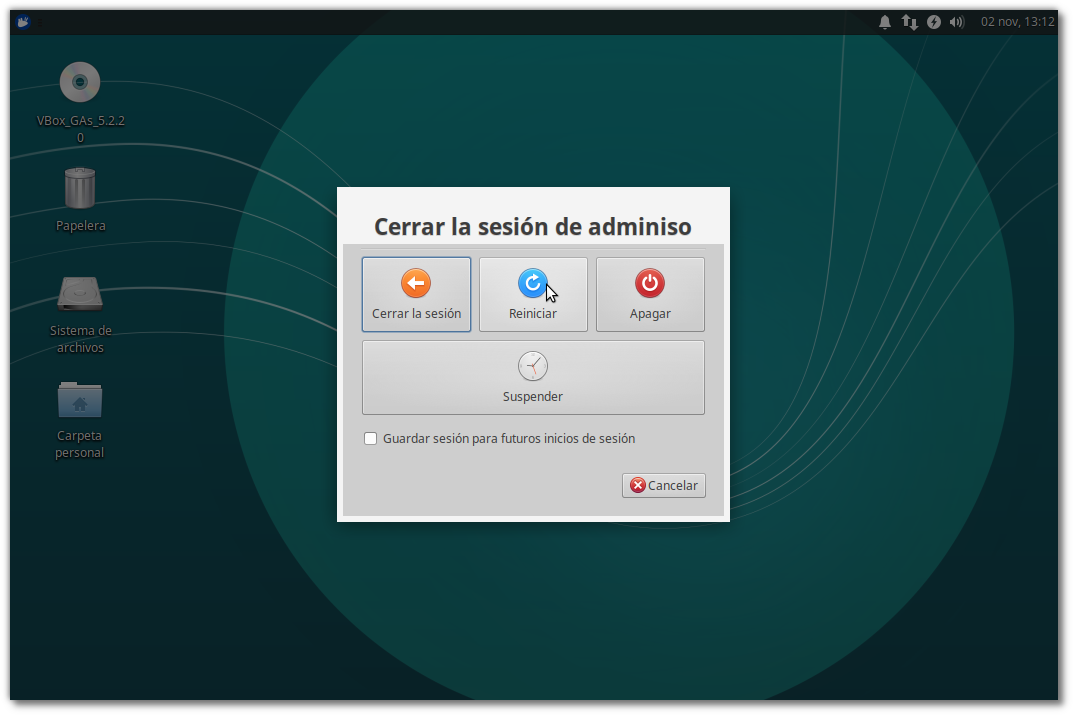
\includegraphics[width=.9\linewidth]{imgs/VBox_GuestAdd_LinuX_026.png}
\end{center}

\subsection{Portapapeles}
\label{sec:org177130d}
Ahora ya tenemos el portapapeles compartido habilitado entre nuestro
hipervisor y la máquina virtual, podemos decidir, la direccionalidad de
este portapapeles.

\begin{itemize}
\item Inhabilitado
\item Hipervisor \(\rightarrow\) MV
\item MV \(\leftarrow\) Hipervisor
\item MV \(\leftrightarrow\) Hipervisor
\end{itemize}

Esto nos será muy útil para seguir manuales, buscar errores en Internet
cuando la máquina virtualizada no tenga conexión o cuando no tengamos el
navegador abierto, para la elaboración de documentación, etc.

\begin{center}
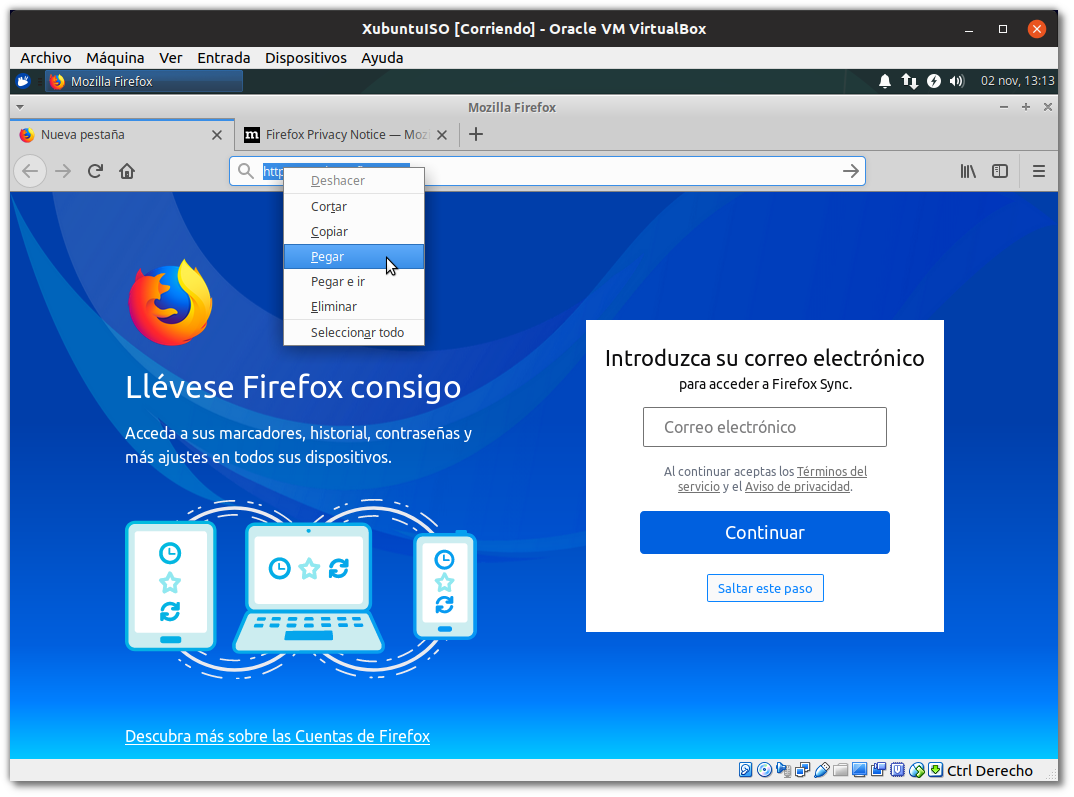
\includegraphics[width=.9\linewidth]{imgs/VBox_GuestAdd_LinuX_027.png}
\end{center}

Realiza todas las configuraciones que hemos visto en la tarea y avisa al
profesor para que compruebe que todo funciona.

\newpag

\newpage

\newpage
\section{Tarea 07 [ CLIL ] : Why is Virtualization Useful?}
\label{sec:org1be2a03}

\begin{center}

\includegraphics[width=50px]{imgs/amongus.png}
\end{center}


Lee el texto que aparece a continuación y contexta a las preguntas:

El texto ha sido extraido del Manual de VirtualBox:
\url{https://www.virtualbox.org/manual/ch01.html\#virt-why-useful}



\newpage 

---
 The techniques and features that Oracle VM VirtualBox provides are useful
 in the following scenarios:

\begin{itemize}
\item \textbf{Running multiple operating systems simultaneously}
Oracle VM VirtualBox enables you to run more than one OS at a time. This way, you can run software written for one OS on another, such as Windows software on Linux or a Mac, without having to reboot to use it. Since you can configure what kinds of virtual hardware should be presented to each such OS, you can install an old OS such as DOS or OS/2 even if your real computer's hardware is no longer supported by that OS.
\item \textbf{Easier software installations} 
Software vendors can use virtual machines to ship entire software configurations. For example, installing a complete mail server solution on a real machine can be a tedious task. With Oracle VM VirtualBox, such a complex setup, often called an appliance, can be packed into a virtual machine. Installing and running a mail server becomes as easy as importing such an appliance into Oracle VM VirtualBox.
\item \textbf{Testing and disaster recovery} 
Once installed, a virtual machine and its virtual hard disks can be considered a container that can be arbitrarily frozen, woken up, copied, backed up, and transported between hosts.
On top of that, with the use of another Oracle VM VirtualBox feature called snapshots, one can save a particular state of a virtual machine and revert back to that state, if necessary. This way, one can freely experiment with a computing environment. If something goes wrong, such as problems after installing software or infecting the guest with a virus, you can easily switch back to a previous snapshot and avoid the need of frequent backups and restores.
Any number of snapshots can be created, allowing you to travel back and forward in virtual machine time. You can delete snapshots while a VM is running to reclaim disk space.
\item \textbf{Infrastructure consolidation}
Virtualization can significantly reduce hardware and electricity costs. Most of the time, computers today only use a fraction of their potential power and run with low average system loads. A lot of hardware resources as well as electricity is thereby wasted. So, instead of running many such physical computers that are only partially used, one can pack many virtual machines onto a few powerful hosts and balance the loads between them.
\end{itemize}
---
\newpage

\begin{enumerate}
\item Realiza un listado de las palabras que no conoces su significado.
\item ¿Qué significa la expresión : \emph{ship entire software configurations}.?
\item Explica la frase: \emph{a virtual machine and its virtual hard disks can be considered a container that can be arbitrarily frozen, woken up, copied, backed up, and transported between hosts}.
\item ¿Qué nos aportan los \emph{snapshots}?.¿Qué recursos del \emph{anfitrión} utilizan?
\item En el último punto (\emph{Infraestructure consolidation}), explica en castellano porqué
las Herramientas de Virtualización pueden reducir el uso de los recursos energéticos.
\end{enumerate}
\end{document}
